\documentclass[12pt]{article}
\usepackage{enumerate}
\usepackage{mathematics}

\DeclareMathOperator{\diam}{\mathrm{diam}}


\begin{document}

\title{Oxford M5 - Multivariable Calculus
  \footnotetext{\url{https://courses.maths.ox.ac.uk/node/5652}}}
\author{}
\date{}
\maketitle


\section{}

\begin{mdframed}
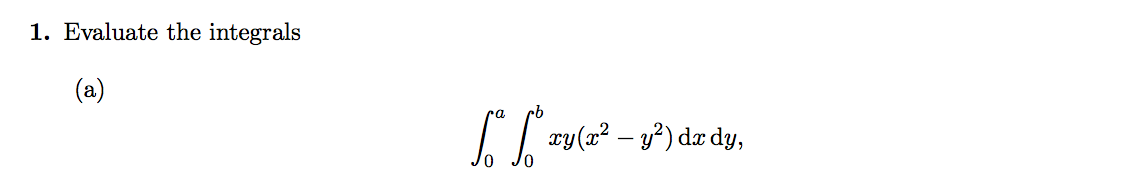
\includegraphics[width=400pt]{img/oxford-prelims-M5-multivariable-calc-1-1-a.png}
\end{mdframed}

\begin{align*}
  \int_0^a\int_0^b xy(x^2 - y^2)\dx\dy
  &= \int_0^a\int_0^b x^3y - xy^3\dx\dy\\
  &= \int_0^a\frac{b^4}{4}y - \frac{b^2}{2}y^3\dy\\
  &= \frac{a^2b^4}{8} - \frac{a^4b^2}{8} \checkmark
\end{align*}

\newpage
\begin{mdframed}
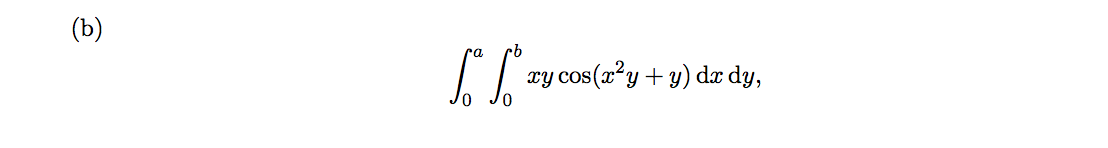
\includegraphics[width=400pt]{img/oxford-prelims-M5-multivariable-calc-1-1-b.png}
\end{mdframed}

Let $u = x^2$ so that $\dxdu = \frac{1}{2x}$. Then

\begin{align*}
  \int_0^a\int_0^b xy\cos(x^2y + y)\dx\dy
  &= \int_0^a\int_0^b xy\cos(uy + y)\dxdu \du\dy\\
  &= \frac{1}{2}\int_0^a\int_{x=0}^{x=b} y\cos(uy + y) \du\dy\\
  &= \frac{1}{2}\int_0^a\Big[\sin(uy + y) \Big]_{u=0}^{u=b^2}\dy\\
  &= \frac{1}{2}\int_0^a\Big[\sin(y(b^2 + 1)) - \sin(y)\Big]\dy\\
  &= \frac{1}{2}\Big[\frac{-\cos(y(b^2 + 1))}{b^2 + 1} + \cos(y)\Big]_{y=0}^{y=a}\\
  &= \frac{1}{2}\Big[\frac{-\cos(a(b^2 + 1))}{b^2 + 1} + \cos(a) +
                     \frac{1}{b^2 + 1} - 1 \Big]\\
  &= \frac{1}{2}\Big[\frac{1 -\cos(a(b^2 + 1))}{b^2 + 1} + \cos(a) - 1 \Big]\\
  &= \frac{1}{2}\Big[\cos(a) - \frac{b^2 + \cos(a(b^2 + 1))}{b^2 + 1} \Big]. \checkmark
\end{align*}

\newpage
\begin{mdframed}
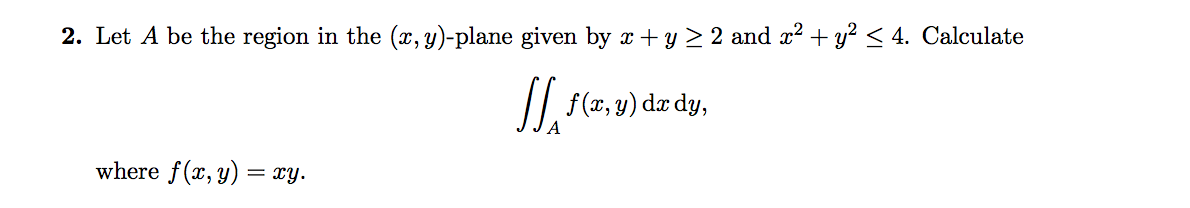
\includegraphics[width=400pt]{img/oxford-prelims-M5-multivariable-calc-1-2.png}
\end{mdframed}
\begin{align*}
     \int_0^2 \int_{2 - x}^{\sqrt{4 - x^2}} xy \dy \dx
  &= \frac{1}{2}\int_0^2 \Big[xy^2\Big]_{y=2 - x}^{y=\sqrt{4 - x^2}} \dx\\
  &= \frac{1}{2}\int_0^2 \Big[x(4 - x^2) - x(2 - x)^2\Big] \dx\\
  &= \frac{1}{2}\int_0^2 x(2-x)\Big[(2 + x) - (2 - x)\Big] \dx\\
  &= \frac{1}{2}\int_0^2 2x^2(2-x) \dx\\
  &= \int_0^2 2x^2 - x^3 \dx\\
  &= \Big[\frac{2}{3}x^3 - \frac{1}{4}x^4\Big]_0^2 \dx\\
  &= \frac{16}{3} - \frac{16}{4}\\
  &= \frac{64 - 48}{12}\\
  &= \frac{4}{3} \checkmark
\end{align*}


\newpage
\begin{mdframed}
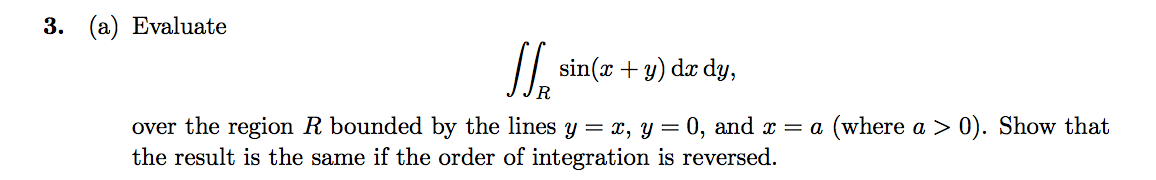
\includegraphics[width=400pt]{img/oxford-prelims-M5-multivariable-calc-1-3-a.png}
\end{mdframed}

\newpage
\begin{mdframed}
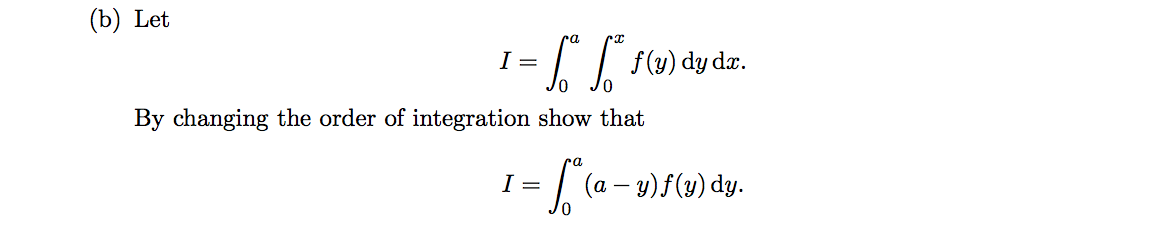
\includegraphics[width=400pt]{img/oxford-prelims-M5-multivariable-calc-1-3-b.png}
\end{mdframed}
\begin{align*}
  \int_0^a\int_0^x f(y) \dy \dx
\end{align*}
\newpage
\begin{mdframed}
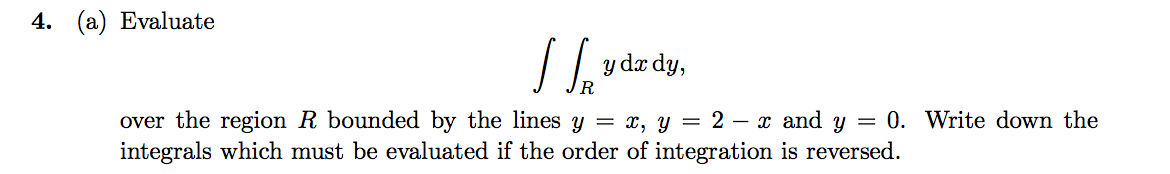
\includegraphics[width=400pt]{img/oxford-prelims-M5-multivariable-calc-1-4-a.png}
\end{mdframed}

\begin{mdframed}
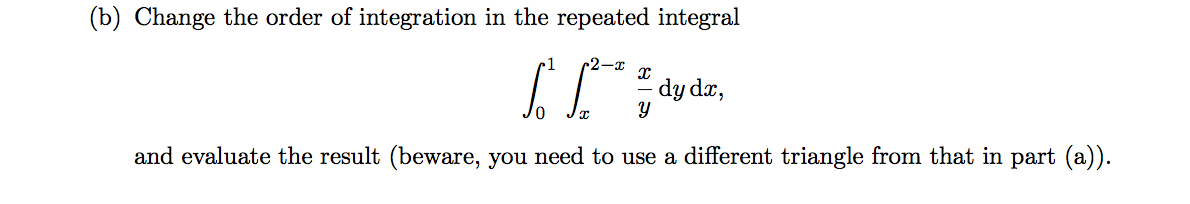
\includegraphics[width=400pt]{img/oxford-prelims-M5-multivariable-calc-1-4-b.png}
\end{mdframed}

\section{}


\end{document}
